\documentclass[11pt,a4paper,french,twoside]{PMCours}
\usepackage{hyperref}
\begin{document}
\TitreISN{Classe de Terminale}{Année 2021--2022}
{Numérique et Science Informatique}{Chap. 6 : Protocoles de routage}
\vskip -.8cm 
Ce chapitre est la suite du chapitre {\bf 5} : {\bf Introduction aux Réseaux}, plus particulièrement de sa section {\bf 2} sur le protocole IP, dont on reprend un extrait ci-dessous. 
\section*{\vskip -.9cm 0 Rappels sur le principe du routage IP}
Dans un réseau, les ordinateurs sont identifiés par leur adresse IP. \\
Les machines sont regroupées en des sous-réseaux, ces sous-réseaux sont eux-même regroupés en des réseaux de taille plus importante,... jusqu'à obtenir Internet, le réseau global. \\
Les (sous-)réseaux sont reliés entre eux par des routeurs, dont le but est de diriger les messages vers leur destination. Plus précisément,

\medskip
\begin{Definition}{}
Le {\color{red}routage} est le mécanisme par lequel des chemins sont sélectionnés dans un réseau pour acheminer les données de l'expéditeur vers le destinataire.  
\end{Definition}

\medskip
L'ordinateur $A$ connaît :
\begin{itemize}
\item sa propre adresse IP;
\item son masque de sous-réseau;
\item et grace à ces données, il connaît donc aussi l'adresse de son sous-réseau $R1$.
\item Une {\em adresse de passerelle} menant à sa passerelle $P1$.
\end{itemize}

$A$ veut envoyer des données à l'ordinateur $Z$ dont il connaît l'adresse IP.

$A$ applique alors son masque de sous-réseau à l'adresse IP de $Z$. 
\begin{itemize}
\item si il obtient l'adresse de $R1$, alors $A$ et $Z$ sont tous deux dans $R1$ et la communication se fera de manière directe (les trames sont directement adressées à l'adresse MAC de $Z$,\ldots) 
\item si $A$ et $Z$ ne sont pas sur le même sous-réseau, alors $A$ envoie la trame vers sa passerelle $P1$, typiquement un routeur. 
\end{itemize}
\begin{Definition}{}Un {\color{red} routeur} est un équipement informatique dont le rôle est d'assurer le routage des paquets d'un réseau vers un autre. Il possède donc plusieurs cartes réseaux (appelées ses {\color{red}interfaces}), chacune possédant sa propre adresse IP et étant reliée à un réseau différent. \\
Un routeur crée et maintient une {\color{red} table de routage} qui contient les routes vers les autres réseaux auquel le routeur a accès et une route par défaut vers laquelle il achemine les paquets correspondant à des destinations inconnues. 
\end{Definition}

\medskip
En comparant l'IP de la machine $Z$ avec les différentes IP enregistrées dans sa table, $P1$ saura vers quelle interface (''sortie'') diriger la trame. Typiquement,
\begin{itemize}
\item si $Z$ appartient à un des sous-réseaux directement reliés à $P1$, $Z$ y est envoyé via l'interface reliée à ce sous-réseau. 
\item si $Z$ appartient à un sous-réseau qui est dans la table de routage de $P1$, $Z$ est envoyé vers une seconde passerelle/routeur ou le processus se répétera.
\item Si $Z$ appartient à un sous-réseau inconnu de $P1$, $Z$ est envoyé vers une passerelle par défaut (ou le processus se répétera).
\end{itemize}

\medskip
On comprend donc que des tables de routages sont l'élément principal pour diriger des messages pour opérer le protocole IP.\\
Lorsqu'on fait une simulation de réseau avec quelques machines et quelques routeurs, on peut configurer les tables de routages à la main. \\
Dans la pratique, il s'agirait d'une tâche titanesque et qui devrait être renouvelée sans cesse, si de nouveaux routeurs sont mis en places, si certains tombent en panne, etc... \\
La création et la mise à jour des tables de routage est donc automatisée, dans un processus qui est décentralisé et dynamique.\\
La suite du chapitre est dédiée à deux protocoles créés dans ce but. 
\section*{1 Le Protocole RIP}
\begin{Definition}{Protocole RIP}
    %cSpell:ignore Protocol
Le protocole RIP (Routing Information Protocol) est un protocole de routage visant à minimiser le nombre de routeurs par lequel un message devra transiter.
\end{Definition}

\medskip
Dans ce protocole, chaque routeur transmet de manière périodique à ses voisins les adresses de ses propres voisins et les informations qu'il a reçues par d'autres routeurs. Il indique de plus la distance (exprimée en nombre de routeurs à traverser) entre lui et les diverses adresses. \\
\`A noter que l'on appelle {\color{red} vecteurs de distance} les couples (adresse,distance).
\subsubsection*{Activité 1}
\begin{multicols}{2}%cSpell:disable
Dans le réseau suivant :\\
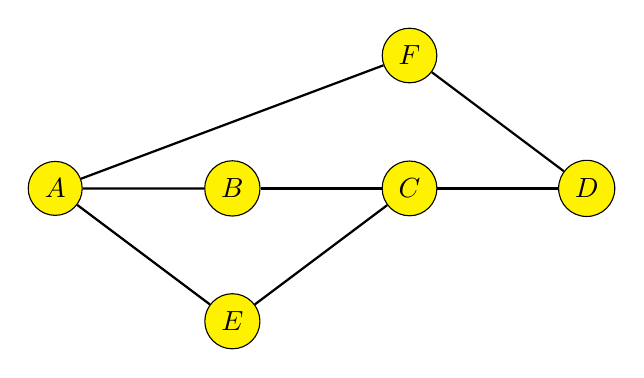
\begin{tikzpicture}[xscale=.75,yscale=.75]
% Styles (MODIFIABLES)
\tikzstyle{fleche}=[-,>=latex,thick]
\tikzstyle{noeud}=[fill=yellow,circle,draw]
\tikzstyle{feuille}=[fill=orange,circle,draw]
% Dimensions (MODIFIABLES)
\def\DistanceInterNiveaux{3}
\def\DistanceInterFeuilles{2}
% Dimensions calculées (NON MODIFIABLES)
\def\NiveauA{(-0)*\DistanceInterNiveaux}
\def\NiveauB{(-.75)*\DistanceInterNiveaux}
\def\NiveauC{(-1.5)*\DistanceInterNiveaux}
\def\NiveauD{(-2.25)*\DistanceInterNiveaux}
\def\InterFeuilles{(.75)*\DistanceInterFeuilles}
% Noeuds (MODIFIABLES : Styles et Coefficients d'InterFeuilles)
\node[noeud] (Rg) at ({(4)*\InterFeuilles},{\NiveauA}) {$F$};
\node[noeud] (Ra) at ({(0)*\InterFeuilles},{\NiveauB}) {$A$};
\node[noeud] (Rb) at ({(2)*\InterFeuilles},{\NiveauB}) {$B$};
\node[noeud] (Rd) at ({(4)*\InterFeuilles},{\NiveauB}) {$C$};
\node[noeud] (Re) at ({(6)*\InterFeuilles},{\NiveauB}) {$D$};
\node[noeud] (Rf) at ({(2)*\InterFeuilles},{\NiveauC}) {$E$};
% Arcs (MODIFIABLES : Styles)
\draw[fleche] (Rg)--(Ra);
\draw[fleche] (Rg)--(Re);
\draw[fleche] (Ra)--(Rb);
\draw[fleche] (Rb)--(Rd);
\draw[fleche] (Rd)--(Re);
\draw[fleche] (Ra)--(Rf);
\draw[fleche] (Rd)--(Rf);
\end{tikzpicture}\\%cSpell:enable
dans lequel le routeur A aurait la table de routage :  

\medskip
\begin{tabular}{|c|c|c|}\hline
Destination&Routeur suivant&Distance\\ \hline
B&B&1\\ \hline
C&B&2\\ \hline
D&F &2 \\ \hline
E&E & 1\\ \hline
F&F &1 \\ \hline
\end{tabular}
\end{multicols}
\begin{multicols}{2}

Table de routage de B : 

\vspace{\stretch{1}}
\begin{tabular}{|c|c|c|}
\hline
Destination&Routeur suivant&Distance\\\hline
&&\\ \hline
&&\\ \hline
&& \\ \hline
&&\\ \hline
&& \\ \hline
\end{tabular}

Table de routage de C :  

\medskip
\begin{tabular}{|c|c|c|}
\hline
Destination&Routeur suivant&Distance\\ \hline
&&\\ \hline
&&\\ \hline
&& \\ \hline
&&\\ \hline
&& \\ \hline
\end{tabular}
\end{multicols}
\subsection*{Description simplifiée du protocole}
On suppose qu'un routeur A reçoit d'un voisin B un vecteur de distance concernant une adresse Z qui est à une distance $d$. (Donc, dans la table de routage de B, on trouve \begin{tabular}{|l|l|l|}\hline Z&??&d \\ \hline \end{tabular} ). Alors, 
\begin{itemize}
\item si Z était inconnue de A, l'information est ajoutée à la table de routage et A vient donc de connaître une destination supplémentaire et le moyen d'y parvenir.\\
On a une nouvelle ligne \begin{tabular}{|l|l|l|}\hline Z&B&d+1 \\ \hline \end{tabular} à la table de routage.\\
{\color{red} En effet, si Z est à une distance $d$ de B et que le chemin de A à Z passe par B, alors A est à une distance d+1 de Z}.
\item si Z était déjà connue de A, alors il y a trois cas à observer :
\begin{itemize}
\item si la route de A à Z passait par un autre voisin C (avec une distance $d'$), alors le vecteur concerne une nouvelle route entre A et Z.

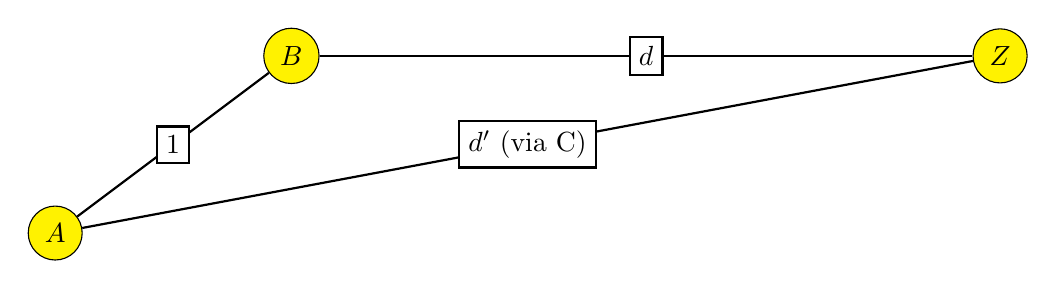
\begin{tikzpicture}[xscale=1,yscale=1]%cSpell:disable
% Styles (MODIFIABLES)
\tikzstyle{fleche}=[-,>=latex,thick]
\tikzstyle{noeud}=[fill=yellow,circle,draw]
\tikzstyle{feuille}=[fill=orange,circle,draw]
\tikzstyle{etiquette}=[midway,fill=white,draw]
% Dimensions (MODIFIABLES)
\def\DistanceInterNiveaux{3}
\def\DistanceInterFeuilles{2}
% Dimensions calculées (NON MODIFIABLES)
\def\NiveauA{(-0)*\DistanceInterNiveaux}
\def\NiveauB{(-.75)*\DistanceInterNiveaux}
\def\NiveauC{(-1.5)*\DistanceInterNiveaux}
\def\NiveauD{(-2.25)*\DistanceInterNiveaux}
\def\InterFeuilles{(.75)*\DistanceInterFeuilles}
% Noeuds (MODIFIABLES : Styles et Coefficients d'InterFeuilles)
\node[noeud] (Ra) at ({(0)*\InterFeuilles},{\NiveauB}) {$A$};
\node[noeud] (Rb) at ({(2)*\InterFeuilles},{\NiveauA}) {$B$};
\node[noeud] (Rz) at ({(8)*\InterFeuilles},{\NiveauA}) {$Z$};
% Arcs (MODIFIABLES : Styles)
\draw[fleche] (Ra)--(Rb) node[etiquette] {$1$};
\draw[fleche] (Rb)--(Rz) node[etiquette] {$d$};
\draw[fleche] (Ra)--(Rz) node[etiquette] {$d'$ (via C)};
\end{tikzpicture}

%cSpell:enable
\begin{itemize}
\item Si la route A-B-Z est plus courte que A-C-Z (c'est-à-dire $1+d<d'$), 
la nouvelle route est meilleure et remplace la précédente. Dans la table de 
routage, désormais, la communication entre A et Z sera dirigée vers B.
La ligne \begin{tabular}{|l|l|l|}\hline Z&B&1+d \\ \hline \end{tabular} 
remplace \begin{tabular}{|l|l|l|}\hline Z&C&d' \\ \hline \end{tabular}.
\item Si la route A-B-Z est plus longue que A-C-Z (c'est-à-dire $1+d\geq d'$), la nouvelle route n'est pas meilleure que la précédente. La table de routage ne sera pas modifiée.\\
On garde la ligne \begin{tabular}{|l|l|l|}\hline Z&C&d' \\ \hline \end{tabular}.
\end{itemize}    
\item si la route de A à Z passait déjà par B, alors on garde bien dans la table de routage la ligne indiquant que la route de A à Z passe par B mais on modifie si il y a lieu la distance. \\
Donc \begin{tabular}{|l|l|l|}\hline Z&B&d \\ \hline \end{tabular} remplace \begin{tabular}{|l|l|l|}\hline Z&B&d'\\ \hline \end{tabular} si $1+d\neq d'$.

\medskip
À noter que si $1+d<d'$, cela signifie que le réseau ''au delà de B'' s'est 
amélioré et un chemin plus court a été trouvé entre B et Z.

Si $1+d>d'$, cela signifie que le réseau ''au delà de B'' s'est détérioré (routeur en panne, liaison saturée) et le chemin entre B et Z est désormais plus long.

Si $1+d=d'$, la mise à jour est inutile et du point de vue de A, le réseau est stable.
\end{itemize}
\end{itemize}
On peut de plus noter que :
\begin{itemize}
\item dans le protocole RIP, la distance maximale autorisée est de 15 et donc on ne peut utiliser ce protocole que pour des réseaux de petites tailles.  
\item si un sous-réseau auparavant accessible devient inaccessible, il est associé à une distance de 16 dans les vecteurs de distance.   
\item pour éviter que des boucles de routage ne puissent se créer, d'autres règles existent. Par exemple, un routeur ne renvoie pas comme information à un un routeur voisin si il a appris cette information de ce même voisin, etc...   
\end{itemize}
%cSpell:ignore OSPF,shortest
\section*{2 Le Protocole OSPF}
Le protocole RIP cherche à minimiser le nombre de routeurs qu'un message devra traverser pour arriver à destination. Mais il ne tient donc absolument pas compte de la nature et de la qualité des liaisons elles-mêmes (fibre optique vs ADSL vs sans fil vs... ) et il est de plus limité aux petits réseaux. Pour remédier à cela, on a créé un protocole qui prend en compte la qualité des liaisons.

\medskip
\begin{Definition}{Protocole OSPF}
\begin{enumerate}
\item On appelle {\color{red}bande passante} d'une liaison son débit binaire maximal, exprimée en bits par secondes.\\
\`A chaque liaison, on associe un {\color{red}poids/coût} d'une liaison donnée par la formule 
$$\mbox{coût}=\frac {10^8}{d}$$ 
où $d$ est la bande passante de la liaison (exprimée en bits par seconde).
\item Le protocole OSPF (Open Shortest Path First) est un protocole de routage faisant transiter les messages par les chemins réalisant le coût minimal entre la source et le but. \\
C'est donc un protocole qui vise à faire passer les messages par les routes de ''meilleur débit global'' . \end{enumerate}
\end{Definition}
\subsubsection*{Activité 2}
\begin{multicols}{2}
On se donne  le réseau :

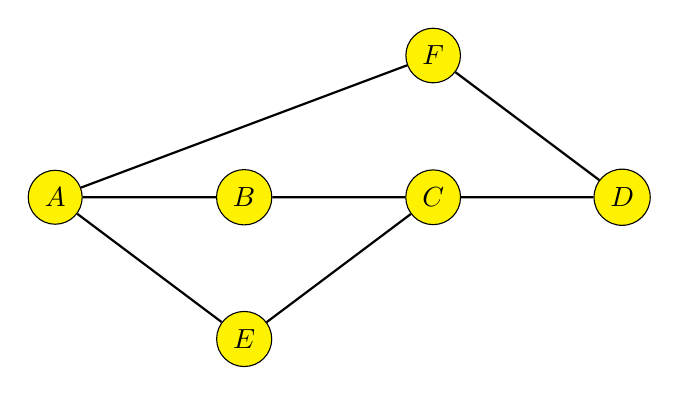
\begin{tikzpicture}[xscale=.8,yscale=.8]%cSpell:disable
% Styles (MODIFIABLES)
\tikzstyle{fleche}=[-,>=latex,thick]
\tikzstyle{noeud}=[fill=yellow,circle,draw]
\tikzstyle{feuille}=[fill=orange,circle,draw]
% Dimensions (MODIFIABLES)
\def\DistanceInterNiveaux{3}
\def\DistanceInterFeuilles{2}
% Dimensions calculées (NON MODIFIABLES)
\def\NiveauA{(-0)*\DistanceInterNiveaux}
\def\NiveauB{(-.75)*\DistanceInterNiveaux}
\def\NiveauC{(-1.5)*\DistanceInterNiveaux}
\def\NiveauD{(-2.25)*\DistanceInterNiveaux}
\def\InterFeuilles{(.75)*\DistanceInterFeuilles}
% Noeuds (MODIFIABLES : Styles et Coefficients d'InterFeuilles)
\node[noeud] (Rg) at ({(4)*\InterFeuilles},{\NiveauA}) {$F$};
\node[noeud] (Ra) at ({(0)*\InterFeuilles},{\NiveauB}) {$A$};
\node[noeud] (Rb) at ({(2)*\InterFeuilles},{\NiveauB}) {$B$};
\node[noeud] (Rd) at ({(4)*\InterFeuilles},{\NiveauB}) {$C$};
\node[noeud] (Re) at ({(6)*\InterFeuilles},{\NiveauB}) {$D$};
\node[noeud] (Rf) at ({(2)*\InterFeuilles},{\NiveauC}) {$E$};
% Arcs (MODIFIABLES : Styles)
\draw[fleche] (Rg)--(Ra);
\draw[fleche] (Rg)--(Re);
\draw[fleche] (Ra)--(Rb);
\draw[fleche] (Rb)--(Rd);
\draw[fleche] (Rd)--(Re);
\draw[fleche] (Ra)--(Rf);
\draw[fleche] (Rd)--(Rf);
\end{tikzpicture}%cSpell:enable

\medskip
dans lequel les liaisons sont de type suivant :
\begin{tabular}{|l|l|l|}\hline
Liaison& Type   & Débit\\\hline
A$\leftrightarrow$B&Modem&50 kbit/s \\\hline
A$\leftrightarrow$E& Wi-Fi&10 Mbit/s       \\\hline
A$\leftrightarrow$F&Fast Ethernet&100 Mbit/s         \\\hline
B$\leftrightarrow$C& Ethernet&10 Mbit/s          \\\hline
C$\leftrightarrow$D&Fibre& 10 Gbit/s         \\\hline
C$\leftrightarrow$E& Bluetooth&5 Mbit/s        \\\hline
D$\leftrightarrow$F& Wi-Fi&1 Gbit/s        \\\hline
\end{tabular}
\end{multicols}
Déterminer le coût de chaque liaison préciser le chemin suivi par un message arrivant au routeur A et à destination d'un sous-réseau attaché au routeur B.

\end{document}
